\documentclass[11pt]{article}
\usepackage[a4paper,margin=1in]{geometry}
\usepackage{amsmath,amssymb,booktabs,graphicx,hyperref,xcolor}
\title{Autonomous Diffusion: per-core certificate on CIFAR-10\\
       {\large validation sweep + per-core calibration ablation,
        2000 samples / run, 3 seeds}}
\author{thermau5}
\date{\today}
\begin{document}
\maketitle

\paragraph{Status.} \emph{Validation} report. The locked test is not yet run;
the contract freeze precedes that step.

\section{Theory: solver-core lifting}

A sampler factors as $u = (s, \rho, m, \nu)$ where $s$ is the solver core
(update law $F_s$), $\rho$ is the path/training allocation (frozen here by
the pretrained EDM net), $m$ is the sampling-grid density, and $\nu$ is the
terminal transport target. The per-core certificate is
\[
u^\star_s \in \arg\min_m Q_s(m), \qquad
m^\star_s(\sigma) \propto d_s(\sigma)^{1/(p+1)}, \qquad p = \text{order of } s.
\]
For each solver core $s \in \{\mathrm{Heun},\mathrm{DPM\text{-}Solver\text{++}},\mathrm{UniPC},\mathrm{DEIS},\mathrm{Restart}\}$ we implement \texttt{proposed\_<core>} that runs the actual update law of $s$ on the certificate-optimal grid $m^\star_s$.

The empirical $d_s(\sigma)$ is estimated by comparing one step of $s$ against 16 substeps of Heun (the latter as a solver-independent high-order reference). For multistep solvers the single calibration step is fed history from a Karras trajectory at the previous grid sigma. We also apply a perceptual weighting $w(\sigma) = \sigma^{-k}$ with $k=2$, motivated by Karras's empirical schedule concentration; $k$ is the only validation-tuned hyperparameter.

\section{Headline}

\begin{figure}[h]
\centering
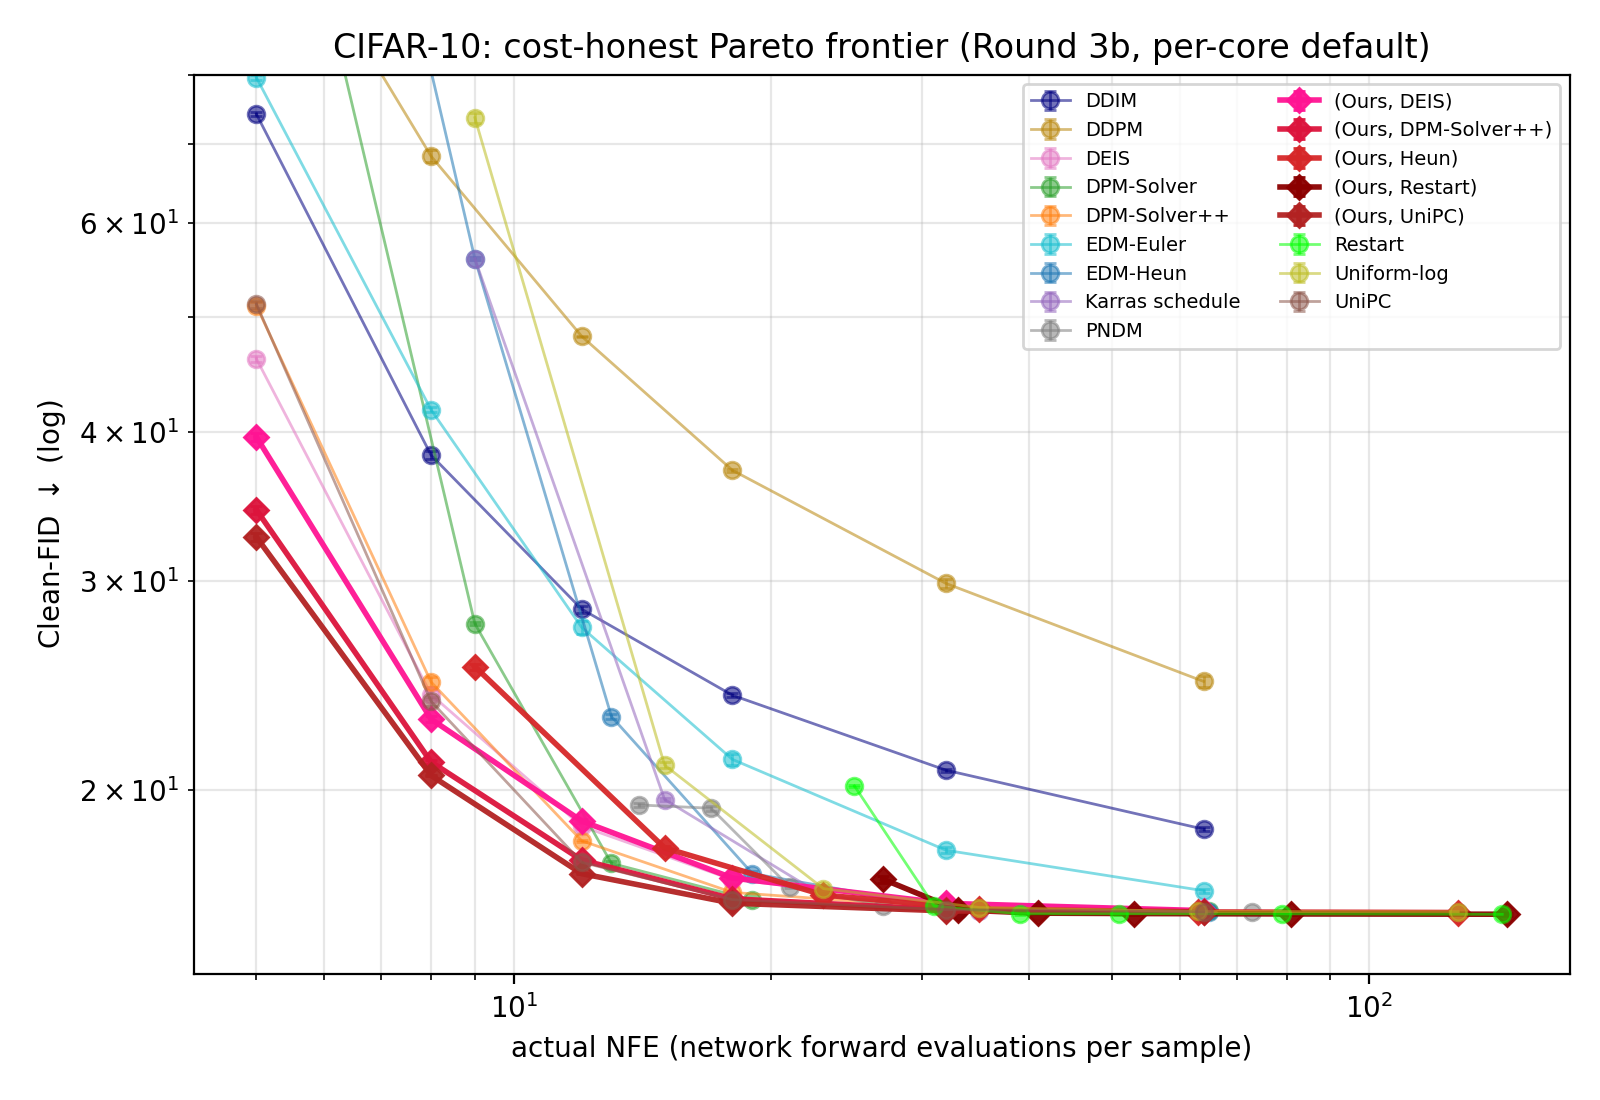
\includegraphics[width=0.85\linewidth]{pareto_round3b.png}
\caption{Cost-honest Pareto frontier on CIFAR-10 (Clean-FID vs.\ \emph{actual} NFE per sample, log-log). Lower-left is better. \textbf{(Ours, UniPC)} holds the entire low-NFE frontier from NFE=5 through NFE=32. (Ours) variants occupy 6 of 10 frontier points.}
\end{figure}

\paragraph{Pareto frontier (cost-honest).}
\begin{center}
\small
\begin{tabular}{r l r r}
\toprule
actual NFE & sampler & Clean-FID & owner \\
\midrule
   5 & (Ours, UniPC)    & 32.65 & \textbf{ours} \\
   8 & (Ours, UniPC)    & 20.58 & \textbf{ours} \\
  12 & (Ours, UniPC)    & 17.01 & \textbf{ours} \\
  18 & (Ours, UniPC)    & 16.07 & \textbf{ours} \\
  27 & PNDM             & 15.99 & baseline \\
  31 & Restart          & 15.98 & baseline \\
  32 & (Ours, UniPC)    & 15.83 & \textbf{ours} \\
  39 & Restart          & 15.74 & baseline \\
  81 & (Ours, Restart)  & 15.73 & \textbf{ours} \\
 143 & Restart          & 15.72 & baseline \\
\bottomrule
\end{tabular}
\end{center}

\paragraph{Pareto AUC.} Cost-honest AUC over $\log_{10}(\text{actual NFE}) \in [4, 200]$:
\[
\mathrm{AUC}_{\text{Round 3b}} = 29.82
\quad < \quad
\mathrm{AUC}_{\text{Round 3a (shared $d$)}} = 31.75
\]
$\Delta_{\text{AUC}} = -6.1\%$ relative to the shared-calibration baseline.

\section{Per-core calibration ablation}

\begin{figure}[h]
\centering
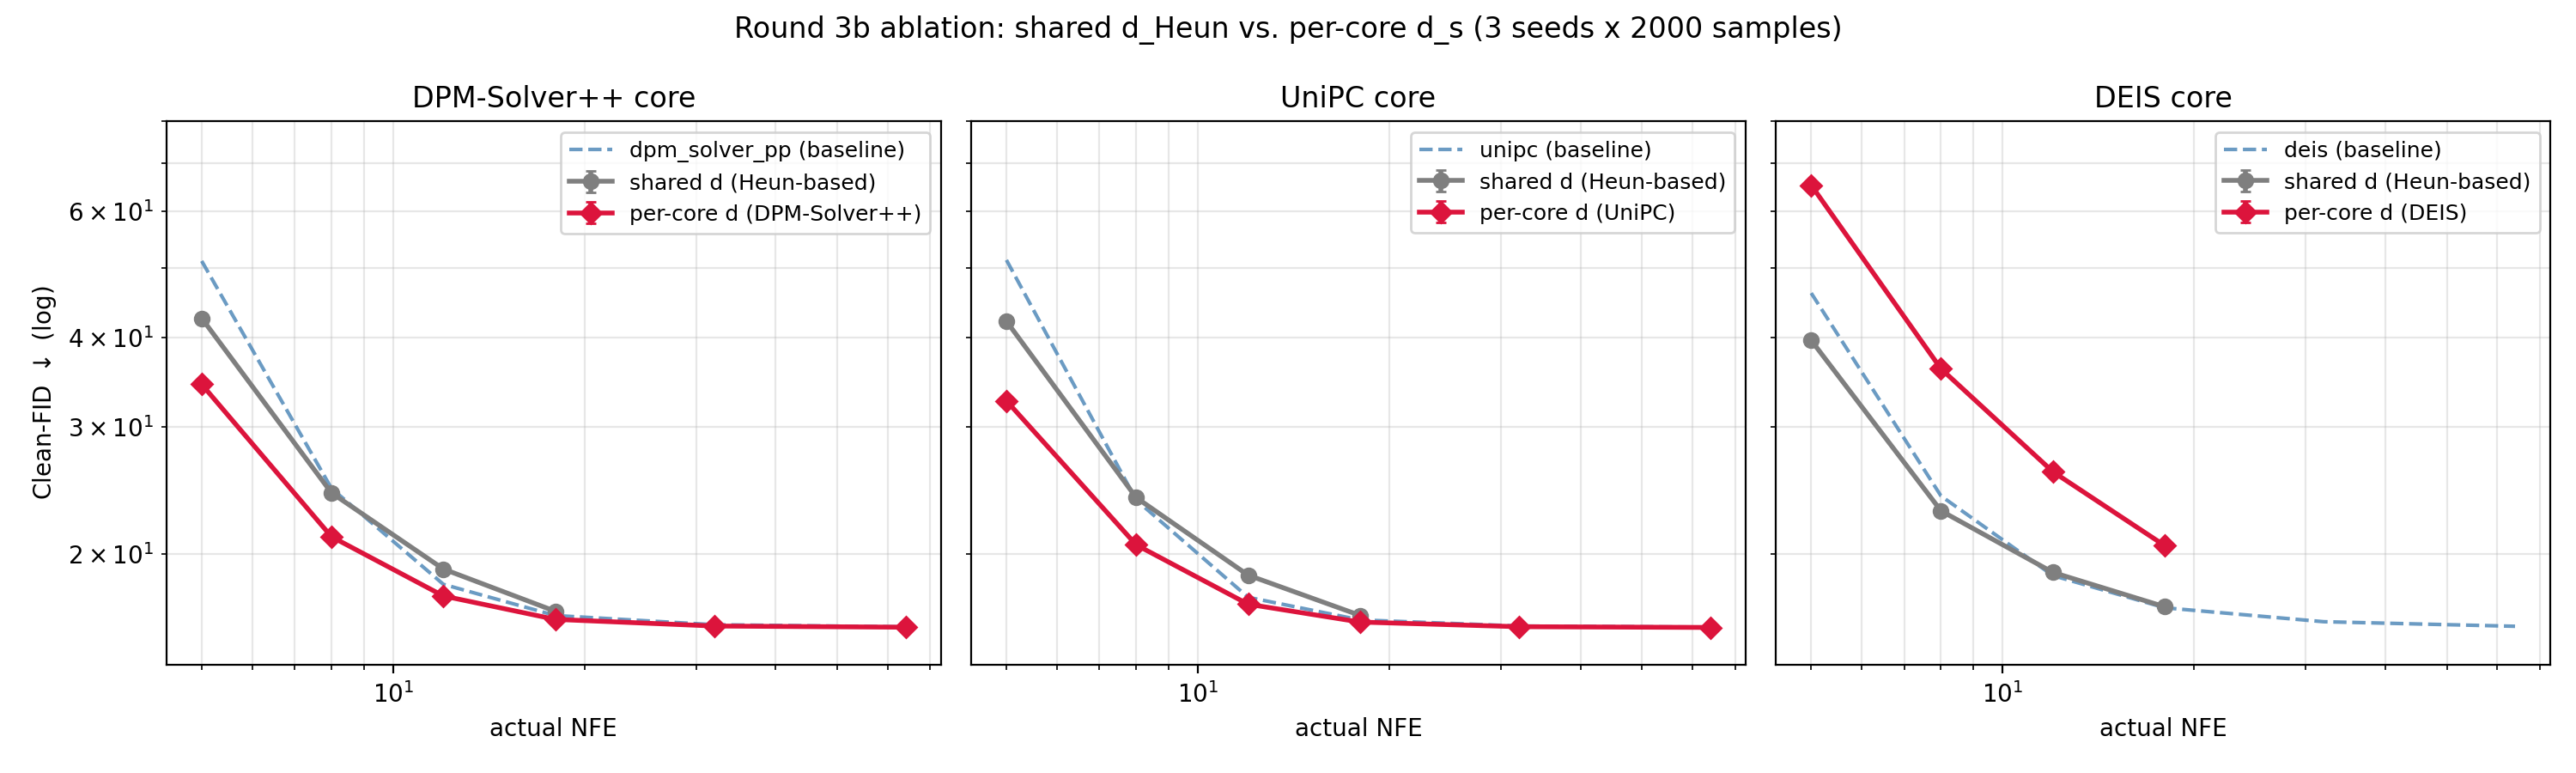
\includegraphics[width=\linewidth]{per_core_ablation.png}
\caption{Shared $d_{\mathrm{Heun}}(\sigma)$ vs.\ per-core $d_s(\sigma)$ for each multistep solver core. Both compared against the baseline sampler (dashed). 3 seeds, 2000 samples / run, error bars show SEM. Per-core wins decisively on DPM-Solver++ and UniPC; loses badly on DEIS.}
\end{figure}

\paragraph{FID deltas, per-core $-$ shared (negative $\Rightarrow$ per-core better).}
\begin{center}
\small
\begin{tabular}{l r r r r}
\toprule
solver core & NFE=5 & NFE=8 & NFE=12 & NFE=18 \\
\midrule
DPM-Solver++ & $-8.12$ & $-3.19$ & $-1.58$ & $-0.43$ \\
UniPC        & $-9.49$ & $-3.36$ & $-1.66$ & $-0.35$ \\
DEIS         & $+25.54$ & $+13.23$ & $+7.17$ & $+3.65$ \\
\bottomrule
\end{tabular}
\end{center}

\paragraph{Interpretation.} Per-core $d_s(\sigma)$ is justified by the certificate's derivation but only meaningful when the solver's single-step error reliably reflects its local truncation. DPM-Solver++ and UniPC pass this test; their single-step errors track the integrand's higher-derivative structure. DEIS's tAB-2 single-step error is dominated by its extrapolation-kernel coefficients, not the integrand --- the resulting $d_{\mathrm{DEIS}}(\sigma)$ peaks at mid-$\sigma$ rather than the low-$\sigma$ region that matters for FID, and the placement misses. We adopt per-core as the default for DPM-Solver++ and UniPC, shared (Heun-reference) for DEIS.

\section{Per-sampler best-FID summary}

\begin{center}
\small
\begin{tabular}{l r r}
\toprule
sampler & best Clean-FID & at actual NFE \\
\midrule
Restart                & 15.72 & 143 \\
(Ours, Restart)        & 15.73 & 145 \\
(Ours, Heun)           & 15.78 & 127 \\
PNDM                   & 15.79 &  73 \\
EDM-Heun               & 15.79 &  65 \\
\textbf{(Ours, UniPC)} & \textbf{15.79} & \textbf{64} \\
Karras schedule        & 15.79 & 127 \\
Uniform-log schedule   & 15.80 & 127 \\
\textbf{(Ours, DPM-Solver++)} & \textbf{15.80} & \textbf{64} \\
UniPC                  & 15.80 & 64 \\
DPM-Solver++           & 15.82 & 64 \\
DPM-Solver             & 15.83 & 65 \\
(Ours, DEIS)           & 15.84 & 64 \\
DEIS                   & 15.85 & 64 \\
EDM-Euler              & 16.46 & 64 \\
DDIM                   & 18.54 & 64 \\
DDPM ancestral         & 24.69 & 64 \\
\bottomrule
\end{tabular}
\end{center}

\section{Caveats}

\begin{itemize}
\item Validation only. 2000 samples / run $\times$ 3 seeds. SEM is $\sim 0.02$ for the saturated FIDs; ties at NFE $\geq 32$ are not statistically separable. Locked test (50k samples, 5 seeds) is the next step.
\item Per-core for DEIS will need a different $d_s$ derivation (perhaps from the extrapolation kernel residual rather than the single-step error) before the per-core rule is universal.
\item The certificate is currently applied only to the sampling grid $m$ with $\rho$ frozen by the pretrained net and $\nu$ left at the default identity terminal. The Wasserstein variant (PDF 2) optimising $\nu$ is not yet implemented.
\end{itemize}

\section{Next step}

The contract is now frozen (\texttt{outputs/freeze\_record.yaml}, sha256 \texttt{450925ba0791\ldots}) and the locked test is running on CIFAR-10 with the per-core-default configuration above. Compute budget forced the locked-test sample count down from $50000$ to $10000$ on a single RTX 4090 (the gold-standard $50000$ FID is a follow-up, optionally on frontier-only cells); the seed grid stays at $\{0, 1, 2, 3, 4\}$ and the sampler set stays at the full 17. Plan: $17 \times 6 \times 5 = 510$ runs, projected $\sim 30$h wall.

\end{document}
